\documentclass{beamer}

\usepackage[utf8]{inputenc}
\usepackage[russian]{babel}
\usepackage{latexsym}
\usepackage{hyperref}

\title[Поверхность молекулы]{Поверхность молекулы и поверхность
    контакта молекул: зачем нужны, алгоритмы, сервисы, примеры применения}
\date{2012}
\usetheme{Warsaw}
\usecolortheme{seahorse}

\begin{document}
    \begin{frame}
        \titlepage
    \end{frame}

    \begin{frame}{Цели построения молекулярной поверхности}
        \begin{itemize}
        \item Для вычисления площади поверхности
         % Площадь поверхности контакта двух молекул позволяет оценить
         % их взаимодействие и, следовательно, стабильность комплекса
        \item Для визуализации на поверхности электростатического потенциала,
            гидрофобных областей и других характеристик
         % Помогает предсказывать области белка, взаимодействующие с
         % другими молекулами, проверять корректность моделей
        \item Для выявления полостей, каналов в белке, карманов и т.п.
         % Следовательно, доступных для воды, ионов, лигандов
        \item Для выявления остатков, экспонированных на поверхности белка
         % Если в одном белке область важна для взаимодействия с
         % другой молекулой, то для похожей области в другом белке
         % можно предсказать подобное же взаимодействие
        \item Для поиска сходных областей поверхности
         % расчет энергии сольватации,  симуляция молекулярной динамики, докинг
        \item \dots
        \end{itemize}
    \end{frame}

    \begin{frame}{Типы молекулярной поверхности}
        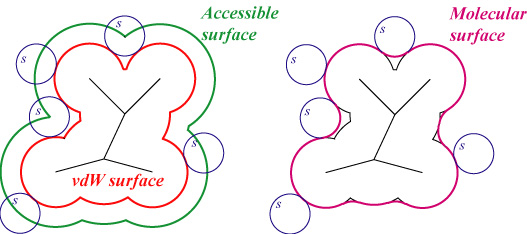
\includegraphics[width=\linewidth]{types.jpg}
        \begin{itemize}
        \item vdWS: Ван-дер-Ваальсова
        \item SAS: доступная для воды
        \item MS: поверхность Коннолли
        \end{itemize}
    \end{frame}

    \begin{frame}{Типы молекулярной поверхности}{vdWS: Ван-дер-Ваальсова}
        \includegraphics[trim=2cm 5cm 2cm 5cm, clip, width=\linewidth]{vdw.png}

        состоит из точек, лежащих на Ван-дер-Ваальсовах сферах атомов молекулы и
        не попадающих внутрь Ван-дер-Ваальсовых сфер других атомов.

        Может содержать сквозные просветы (смотри на рисунке слева).
    \end{frame}

    \begin{frame}{Типы молекулярной поверхности}{SAS: доступная для воды}
        \includegraphics[trim=2cm 5cm 2cm 5cm, clip, width=\linewidth]{sas.png}

        описана центром сферической молекулы воды (радиус 1.4 \AA),
        <<прокатанной>> вокруг атомов белка.
    \end{frame}

    \begin{frame}{Типы молекулярной поверхности}{MS: поверхность Коннолли}
        \includegraphics[trim=2cm 5cm 2cm 5cm, clip, width=\linewidth]{connolly.png}

        описана поверхностями молекул воды, находящимися в контакте с белком;
        <<поверхность, исключаемая растворителем>>:
        поверхность тела, получающегося при исключении из объема точек,
        в которых может находиться растворитель.
    \end{frame}

\end{document}

